\newpage
\section{Results}
% General structure.
% Display spectrums, try to calculate quality factor at least.
% Display some prelimary purities.
% Some stuff I probably should have calculated:
% Powers in the waveguide, peak power
\subsection{Glassgow}



This chip was used to do an initial proof of concept that the JSI of a ring resonator could be measured. Here the aim was to explore different ring geometries and develop an intuition on how to do the experiment. The Pritel pulsed laser was used with a pulse duration of \SI{2}{\pico\second}, a FWHM of \SI{1.0}{\nano\meter} with wavelength range \SI{1530}{\nano\meter} to \SI{1530}{\nano\meter} and a peak power of \SI{100}{\watt}. Due to the laser sometimes destroying the spot size converter on the chip a \SI{3}{\decibel} attenuator was added to just after the laser output.

% b32
\begingroup
    \centering  
    \includegraphics[width=15cm]{/home/luka/Dropbox/cqp/report/thesis/res/glassgow/B32/graph.pdf}
    \captionof{figure}{{\bf JSI Ring B32} We calculate a quality factor of $Q \approx $. In this instance the coupling loss was on average \SI{0}{\deci\bel\m} and the input power of the pulsed laser was \SI{0}{\deci\bel\m} giving a estimated power in waveguide of \SI{0}{\deci\bel\m}. The probe laser operated at \SI{1}{\m\watt}. Fitting the spectral scans of the ring resonators gives coupling parameters of the order $r=0.985$ $\tau = 0.946$ $n_{eff} = 4.136$, note these are only estimates.} 
     \vspace{3pt} \label{crossCompare}
\endgroup
% c21
\begingroup
    \centering  
    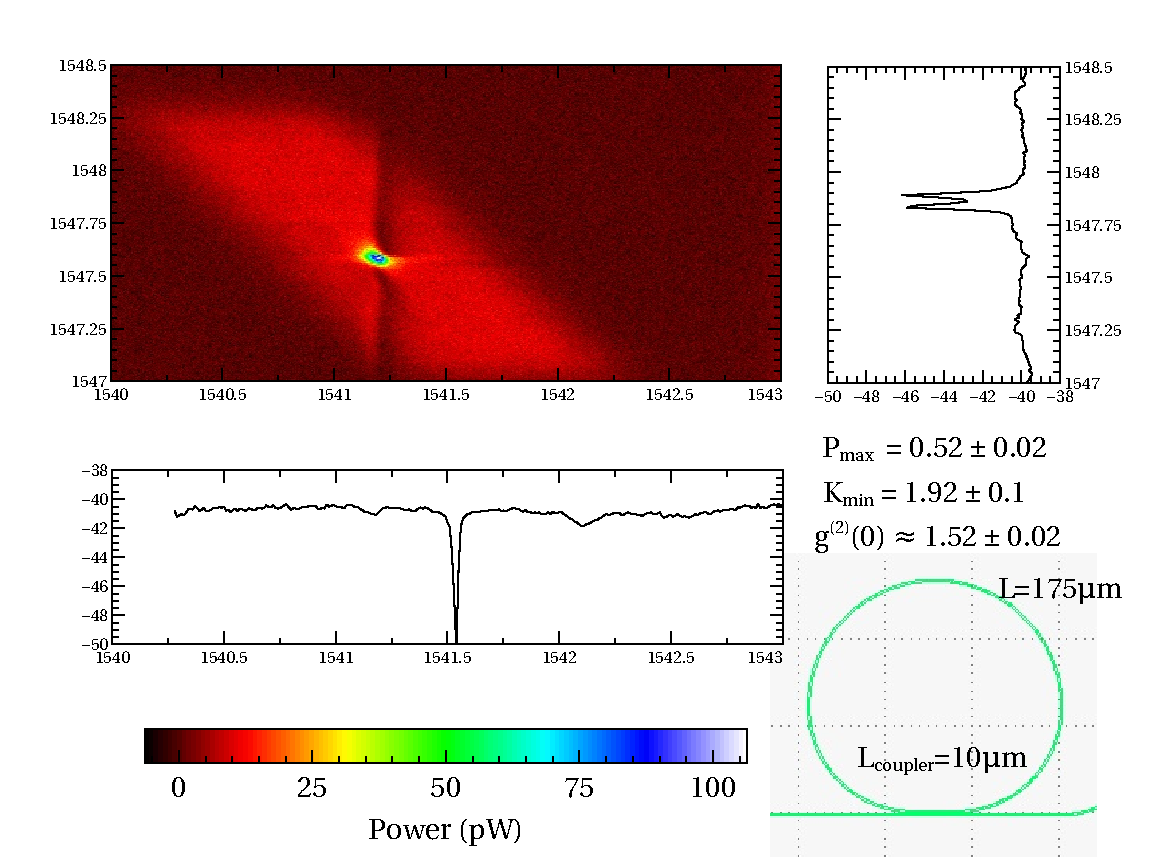
\includegraphics[width=15cm]{/home/luka/Dropbox/cqp/report/thesis/res/glassgow/C21/c21graph.pdf}
    \captionof{figure}{{\bf JSI Ring C21} We calculate a quality factor of $Q \approx 28000$. In this instance the coupling loss was on average \SI{21}{\dB} and the input power of the pulsed laser was \SI{5.5}{\deci\bel\m} giving a estimated power in waveguide of \SI{-5}{\deci\bel\m}. The probe laser operated at \SI{1}{\m\watt}. Fitting the spectral scans of the ring resonators gives coupling parameters of the order $r=0.99$ $\tau = 0.94$ $n_{eff} = 4.144$, note these are only estimates.} 
     \vspace{3pt} \label{crossCompare}
\endgroup
% c17
\begingroup
    \centering  
    \includegraphics[width=15cm]{/home/luka/Dropbox/cqp/report/thesis/res/glassgow/C17/graph.pdf}
    \captionof{figure}{{\bf JSI Ring C17} We calculate a quality factor of $Q \approx 25000$. In this instance the coupling loss was on average \SI{20}{\dB} and the input power of the pulsed laser was \SI{5.1}{\dB} giving a estimated power in waveguide of \SI{-5}{\dB}. The probe laser operated at \SI{1}{\m\watt}. Fitting the spectral scans of the ring resonators gives coupling parameters of the order $r=0.985$ $\tau = 0.946$ $n_{eff} = 4.136$, note these are only estimates.} 
     \vspace{3pt} \label{crossCompare}
\endgroup

\subsection{Toshiba}


\subsubsection{Bistability Data}
% Should be easy
\subsubsection{Pulse shaping}
% Touch on the pulse shaping experiment
\subsubsection{Power Scans}
%
\subsection{a-Si}

% Some initial joint spectrums.
% Try to calculate the quality of the rings.
% Analyse the g2(0) data